\documentclass{article}
\usepackage{graphicx}
\usepackage{amsmath}
\usepackage{fancyhdr}

\setlength{\parindent}{0em}
\setlength{\parskip}{1em}
\renewcommand{\baselinestretch}{1.5}

\pagestyle{fancy}
\fancyhf{}
\lhead{Thank you}
\rfoot{Page \thepage}
\lfoot{text classification}

\title{Text Classification }
\author{Aman Berhe}

\begin{document}
	\maketitle
	\newpage
	\section{Data Preprocessing}
	The following diagram illustrates the main steps\\
	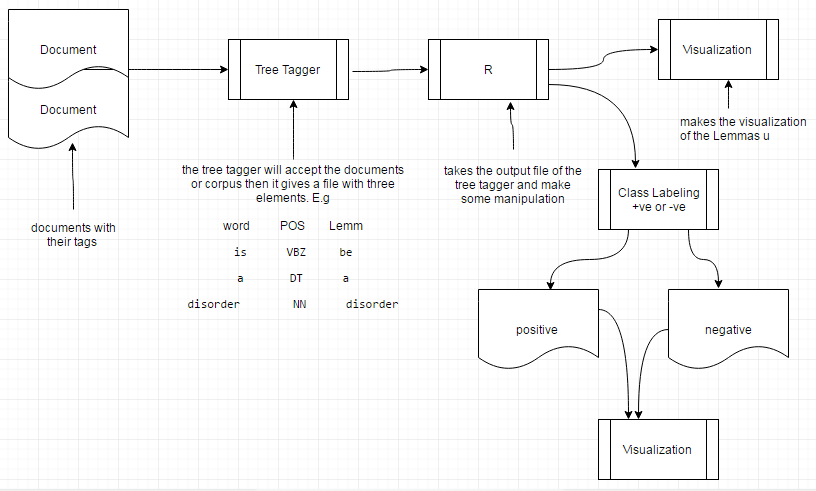
\includegraphics[scale=0.8]{textcl_diagram.PNG}\\   
	As shown in the picture:
	\begin{enumerate} 
		\item Documents\\
		Documents are collected from the website from the page source and then fed to the tree tagger.Currently, I have collected the data for pompe disease of 10 and 30 articles. 
		\item Tree Tagger\\ 
		The tree tagger takes the collected documents and gives an out put file which is three parts: which are word, POS, lemma and the command used was 
		
		cmd/tree-tagger-english 'pompeDatawithtag30' tee ~/outputfile2.txt
		
		\newpage
		E.g: part of output file\\
		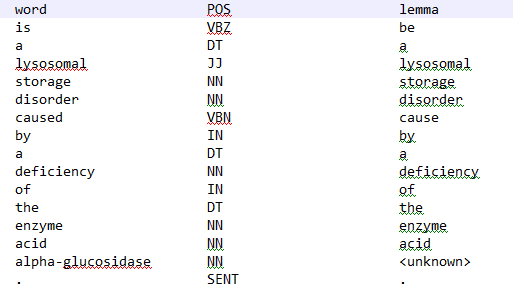
\includegraphics[scale=0.8]{eg.PNG}\\   
		\item Data Manipulation using R
		The output of tree tagger will be used, we will use only the lemmas of the file and visualize the item frequencies.\\
		It is done using the itemfrequencyplot(): which is a function inside the rpart library in R. as well using the item frequency: itemfrequency() and histogram: hist(). 
		
		
		\item Labeling Words\\
		
		The labeling of the sentences into positive and negative is done using SENT POS which indicates the end of a sentence and "$<$span class='symptom'$>$"  which indicates a sentence has a word which is a symptom of a disease.\\
		
	\end{enumerate}
	\end{document}}